\chapter{Parameter Pairs Distributions}\label{appendix:Distributions1}
More plots on \url{https://github.com/RomanKosovnenko/master_thesis/tree/master/images/PairsDistr}
\begin{figure}[!htb]
	\centering
	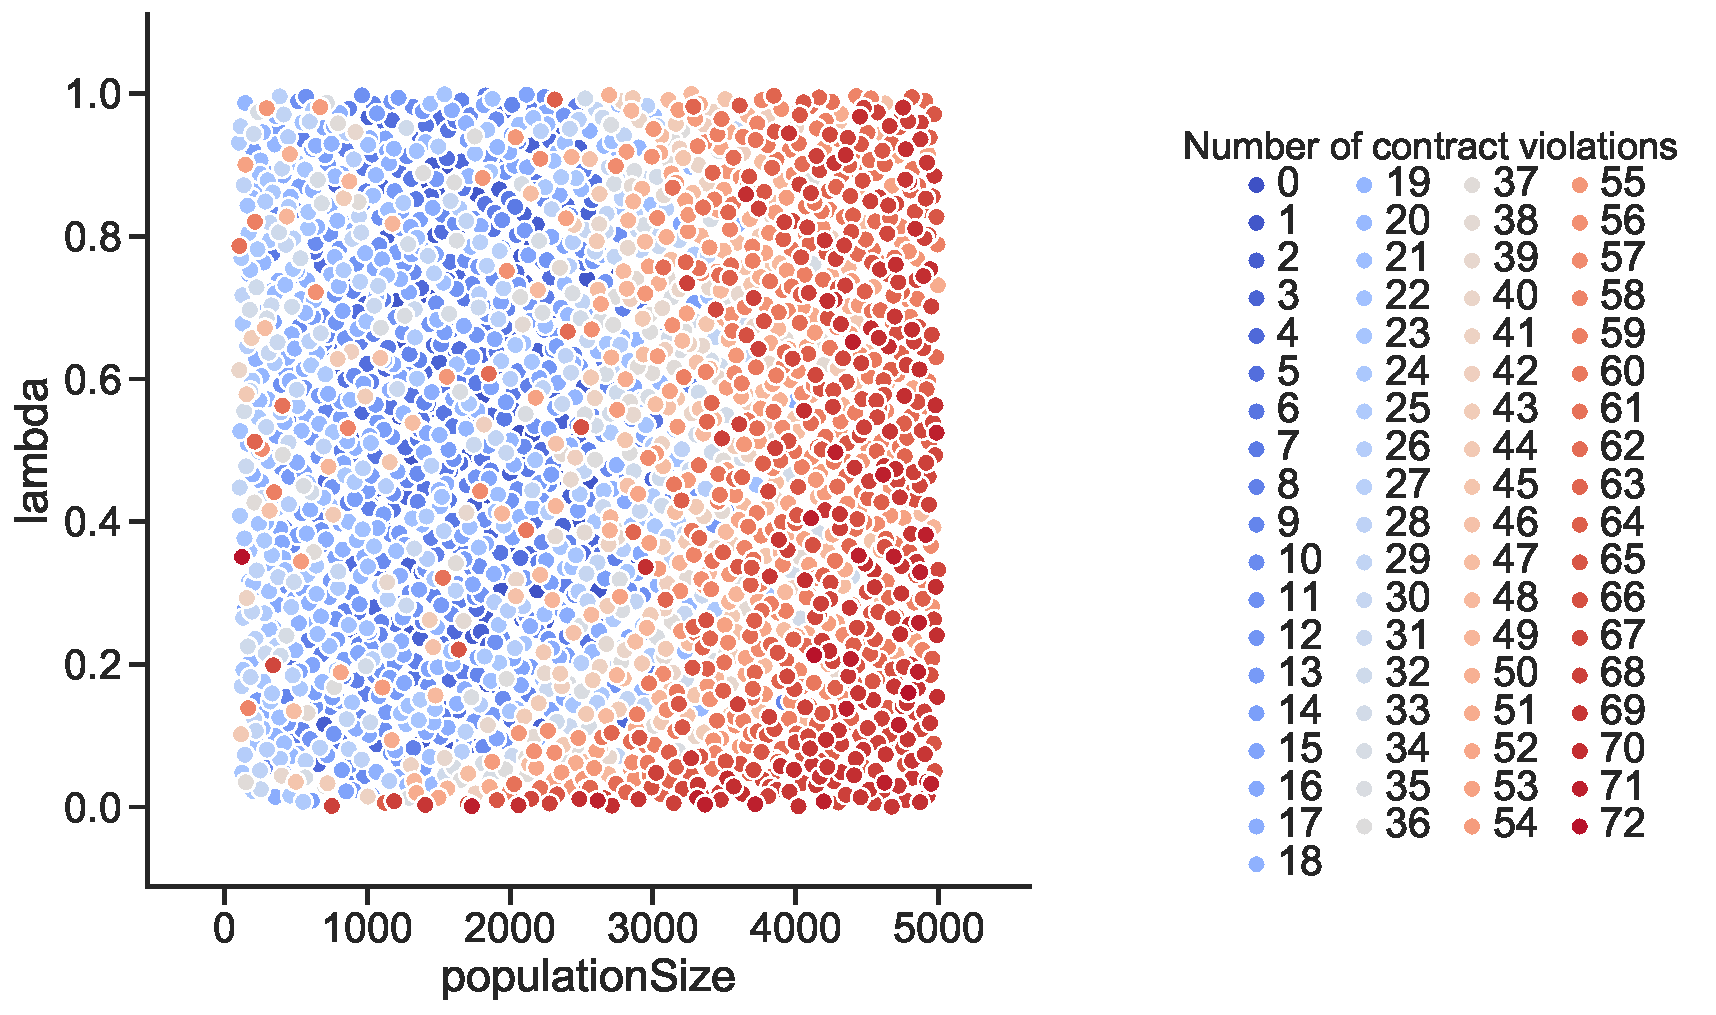
\includegraphics[width=\textwidth]{images/PairsDistr/populationSize_lambda.pdf}
	\caption[]{populationSize and lambda pairs distribution}
	\label{fig:populationSize_lambda_pair}
\end{figure}
\begin{figure}
	\centering
	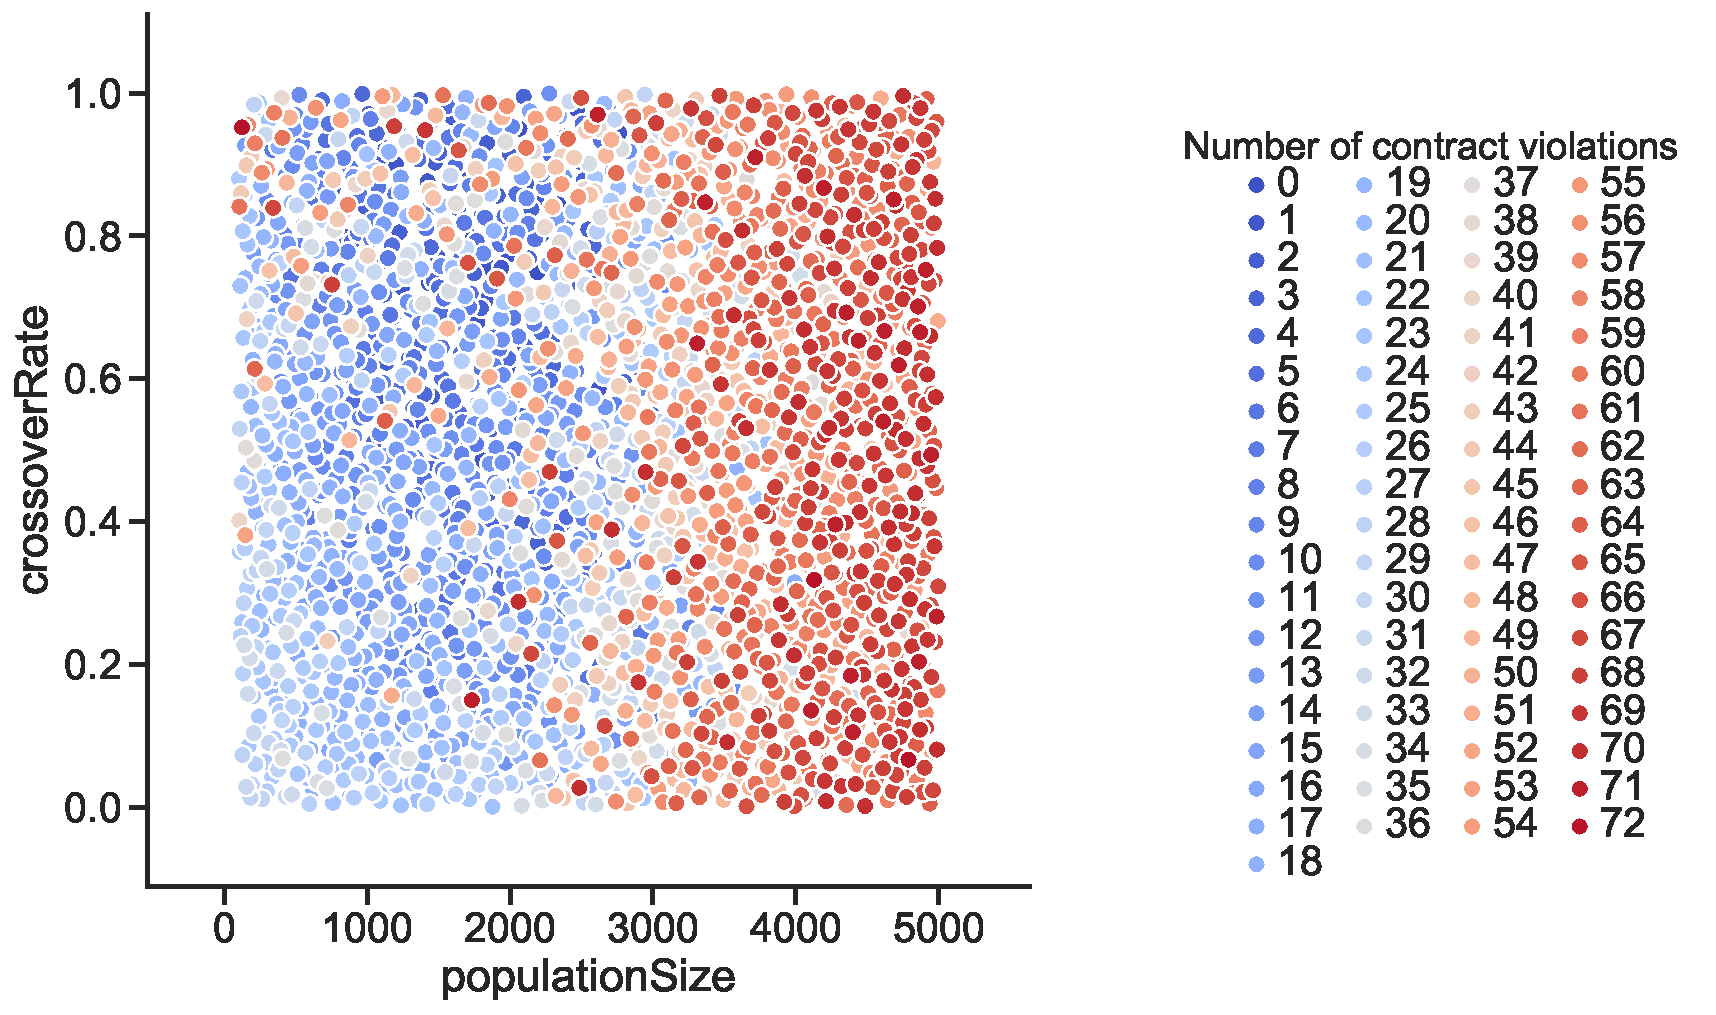
\includegraphics[width=\textwidth]{images/PairsDistr/populationSize_crossoverRate.pdf}
	\caption[]{populationSize and crossoverRate pairs distribution}
	\label{fig:populationSize_crossoverRate_pair}
\end{figure}

\begin{figure}
	\centering
	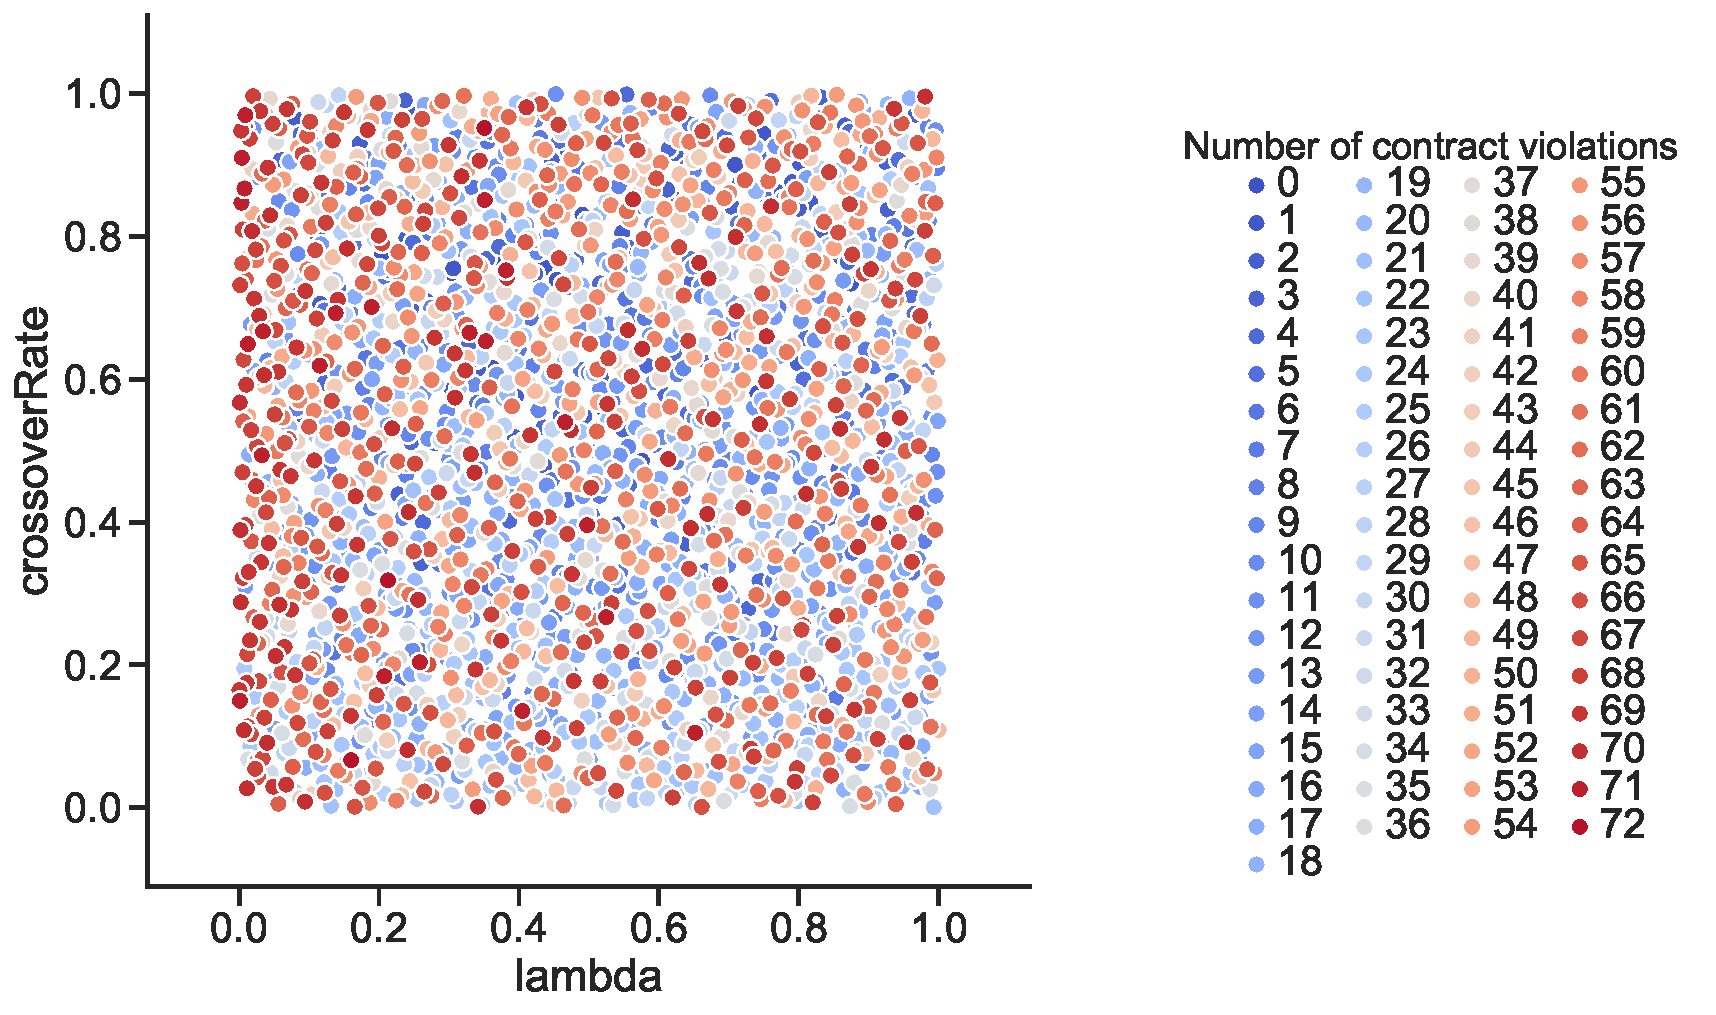
\includegraphics[width=\textwidth]{images/PairsDistr/lambda_crossoverRate.pdf}
	\caption[]{lambda and crossoverRate pairs distribution}
	\label{fig:lambda_crossoverRate_pair}
\end{figure}

\begin{figure}
	\centering
	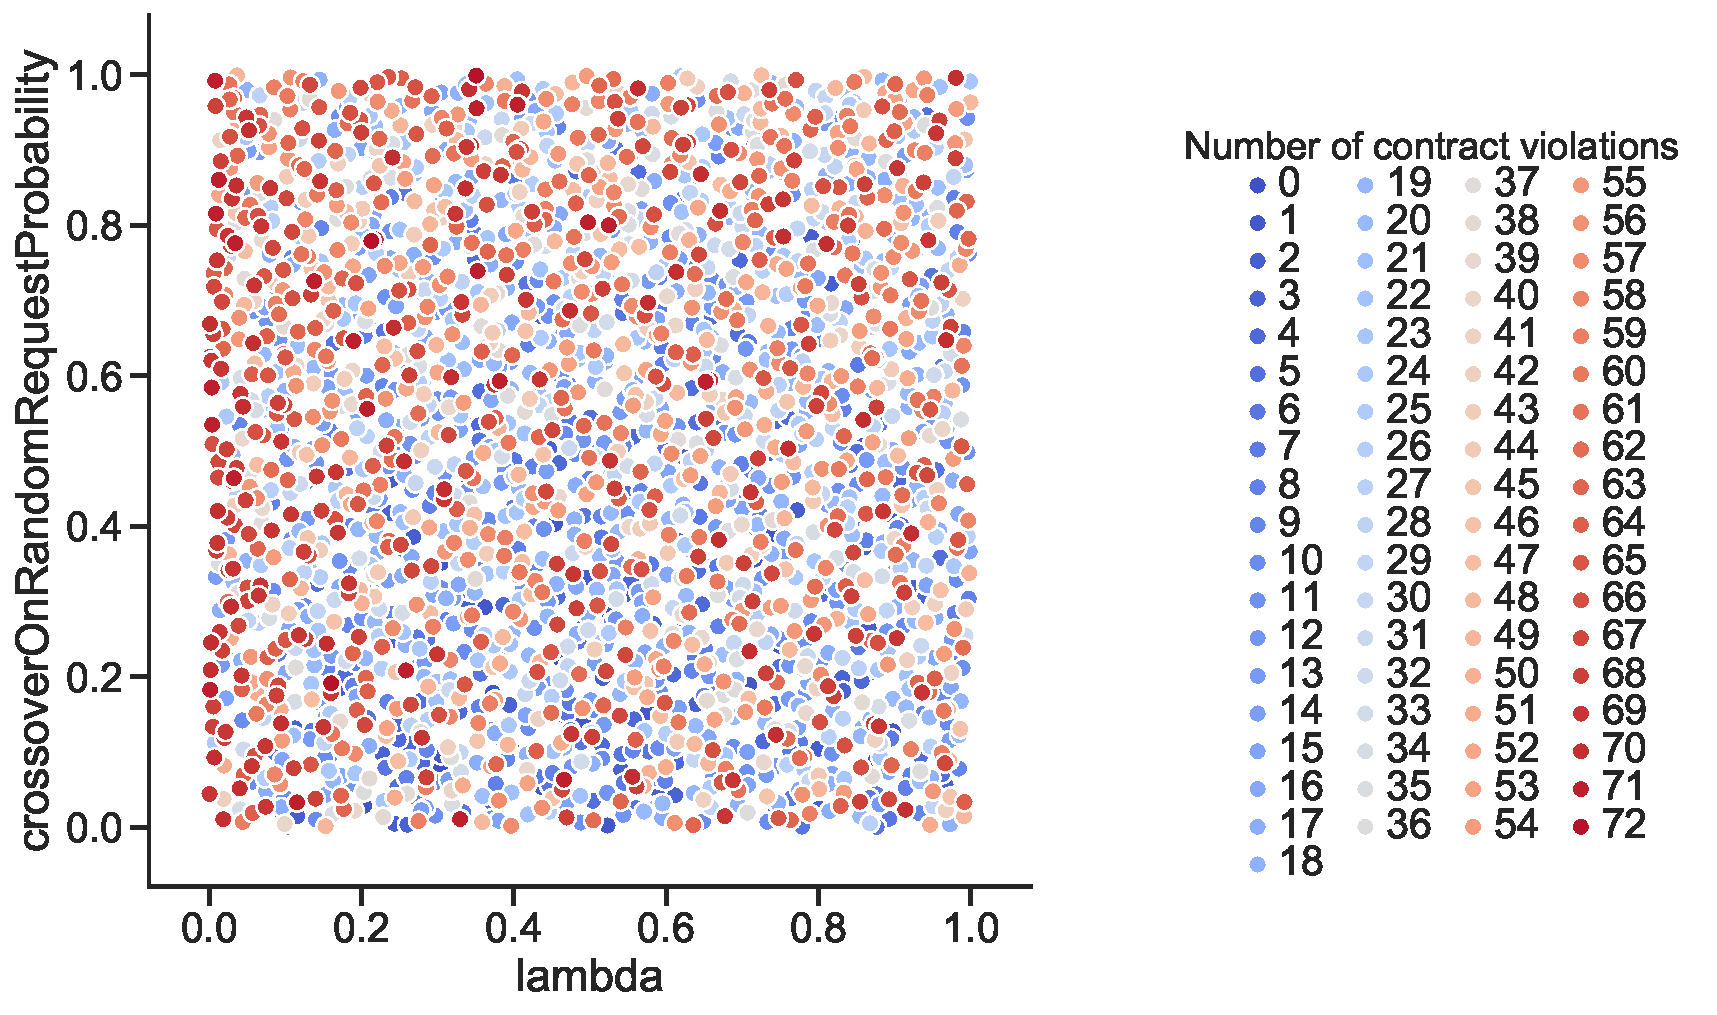
\includegraphics[width=\textwidth]{images/PairsDistr/lambda_crossoverOnRandomRequestProbability.pdf}
	\\caption[]{lambda and crossoverOnRandomRequestProbability pairs distribution}
	\label{fig:lambda_crossoverOnRandomRequestProbability_pair}
\end{figure}

\begin{figure}
	\centering
	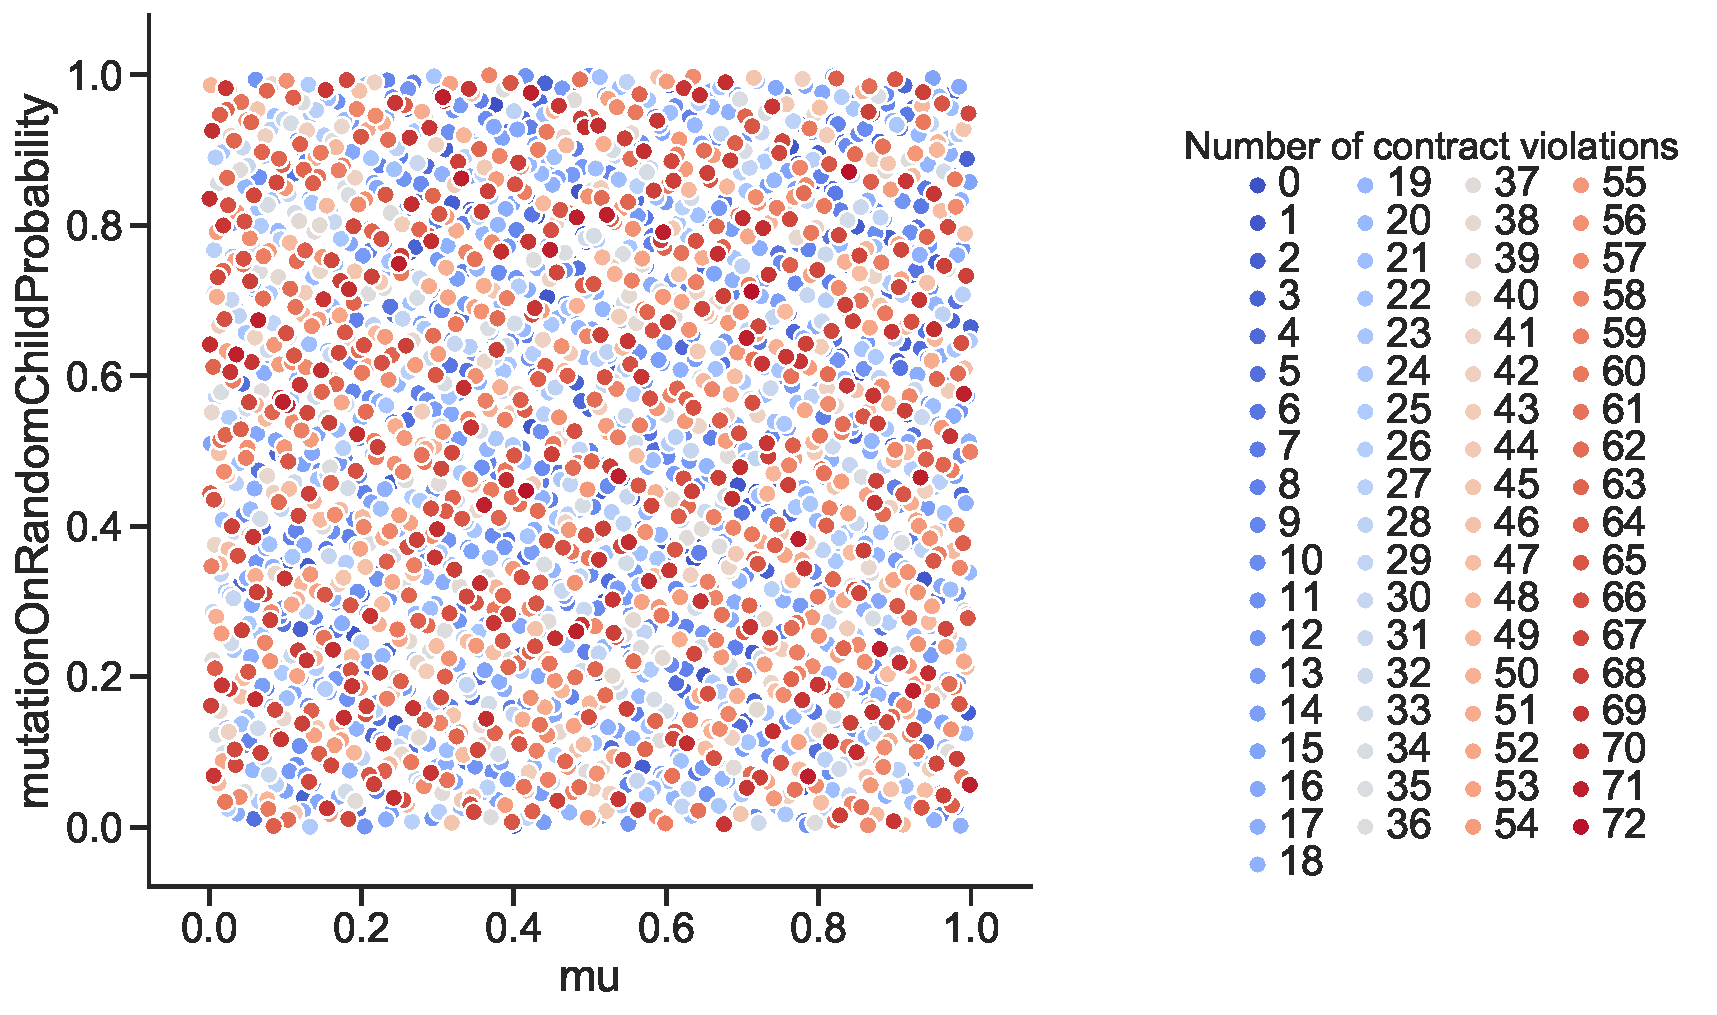
\includegraphics[width=\textwidth]{images/PairsDistr/mu_mutationOnRandomChildProbability.pdf}
	\caption[]{mu and mutationOnRandomChildProbability pairs distribution}
	\label{fig:mu_mutationOnRandomChildProbability_pair}
\end{figure}


\begin{figure}
	\centering
	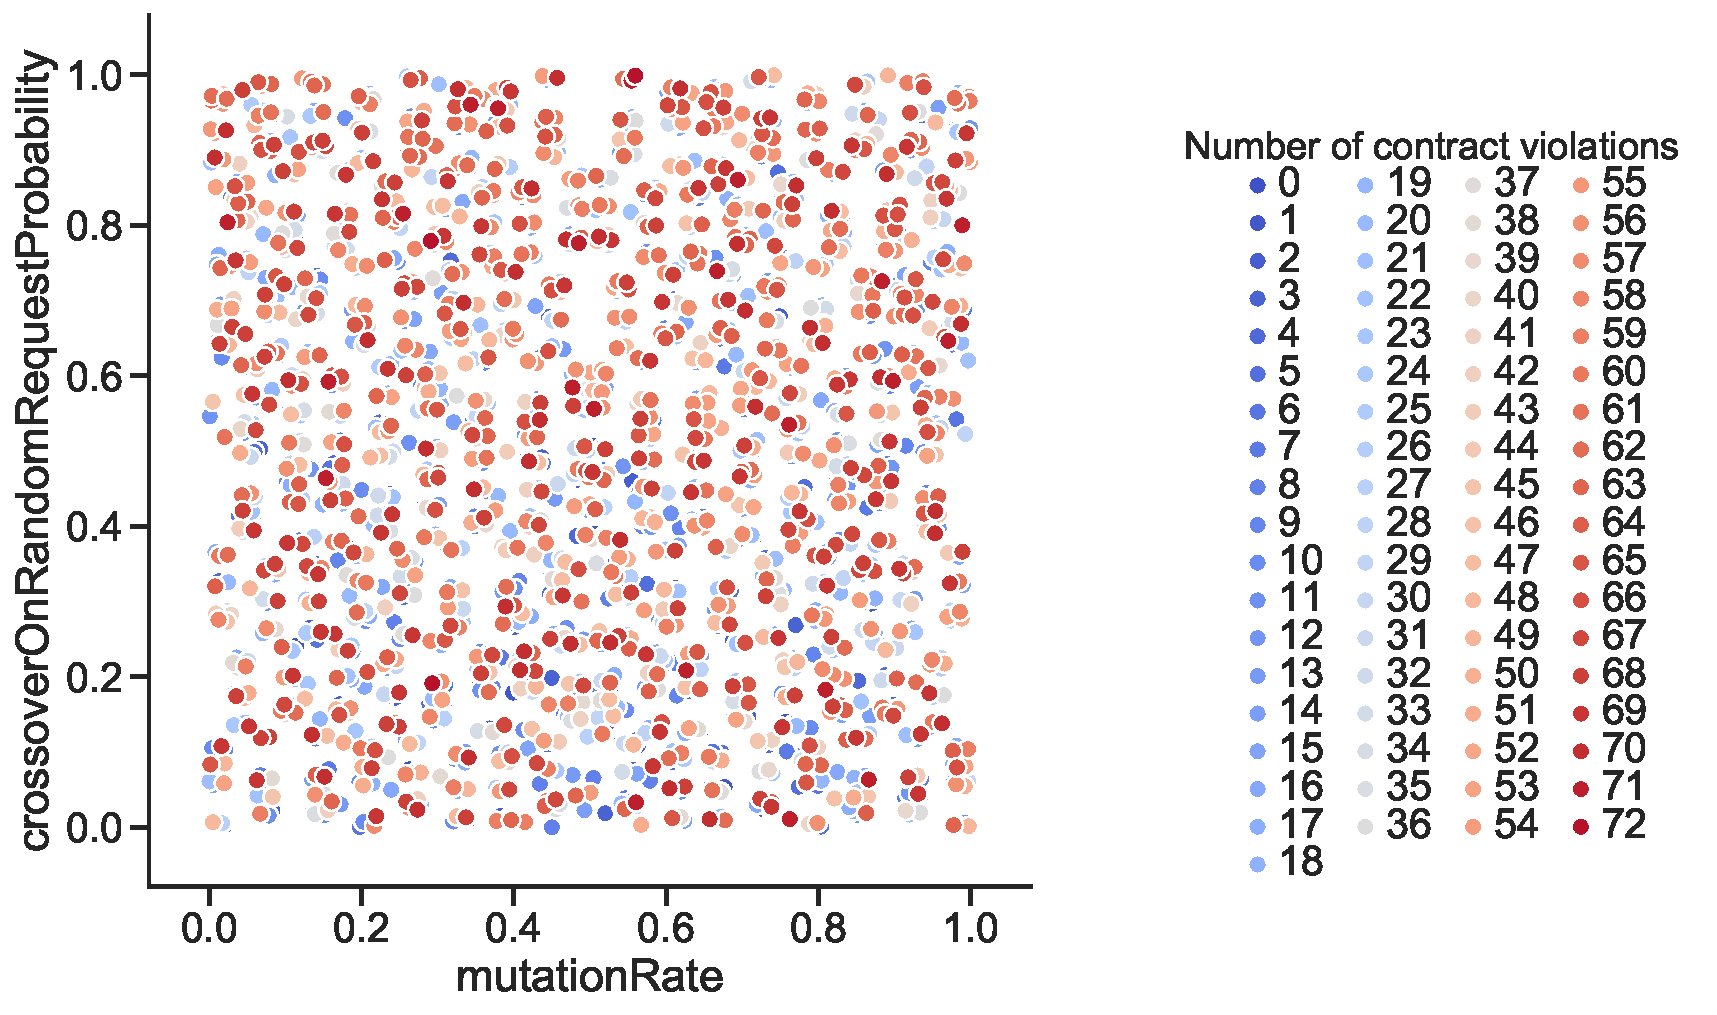
\includegraphics[width=\textwidth]{images/PairsDistr/mutationRate_crossoverOnRandomRequestProbability.pdf}
	\caption[]{mutationRate and crossoverOnRandomRequestProbability pairs distribution}
	\label{fig:mutationRate_crossoverOnRandomRequestProbability_pair}
\end{figure}


\begin{figure}
	\centering
	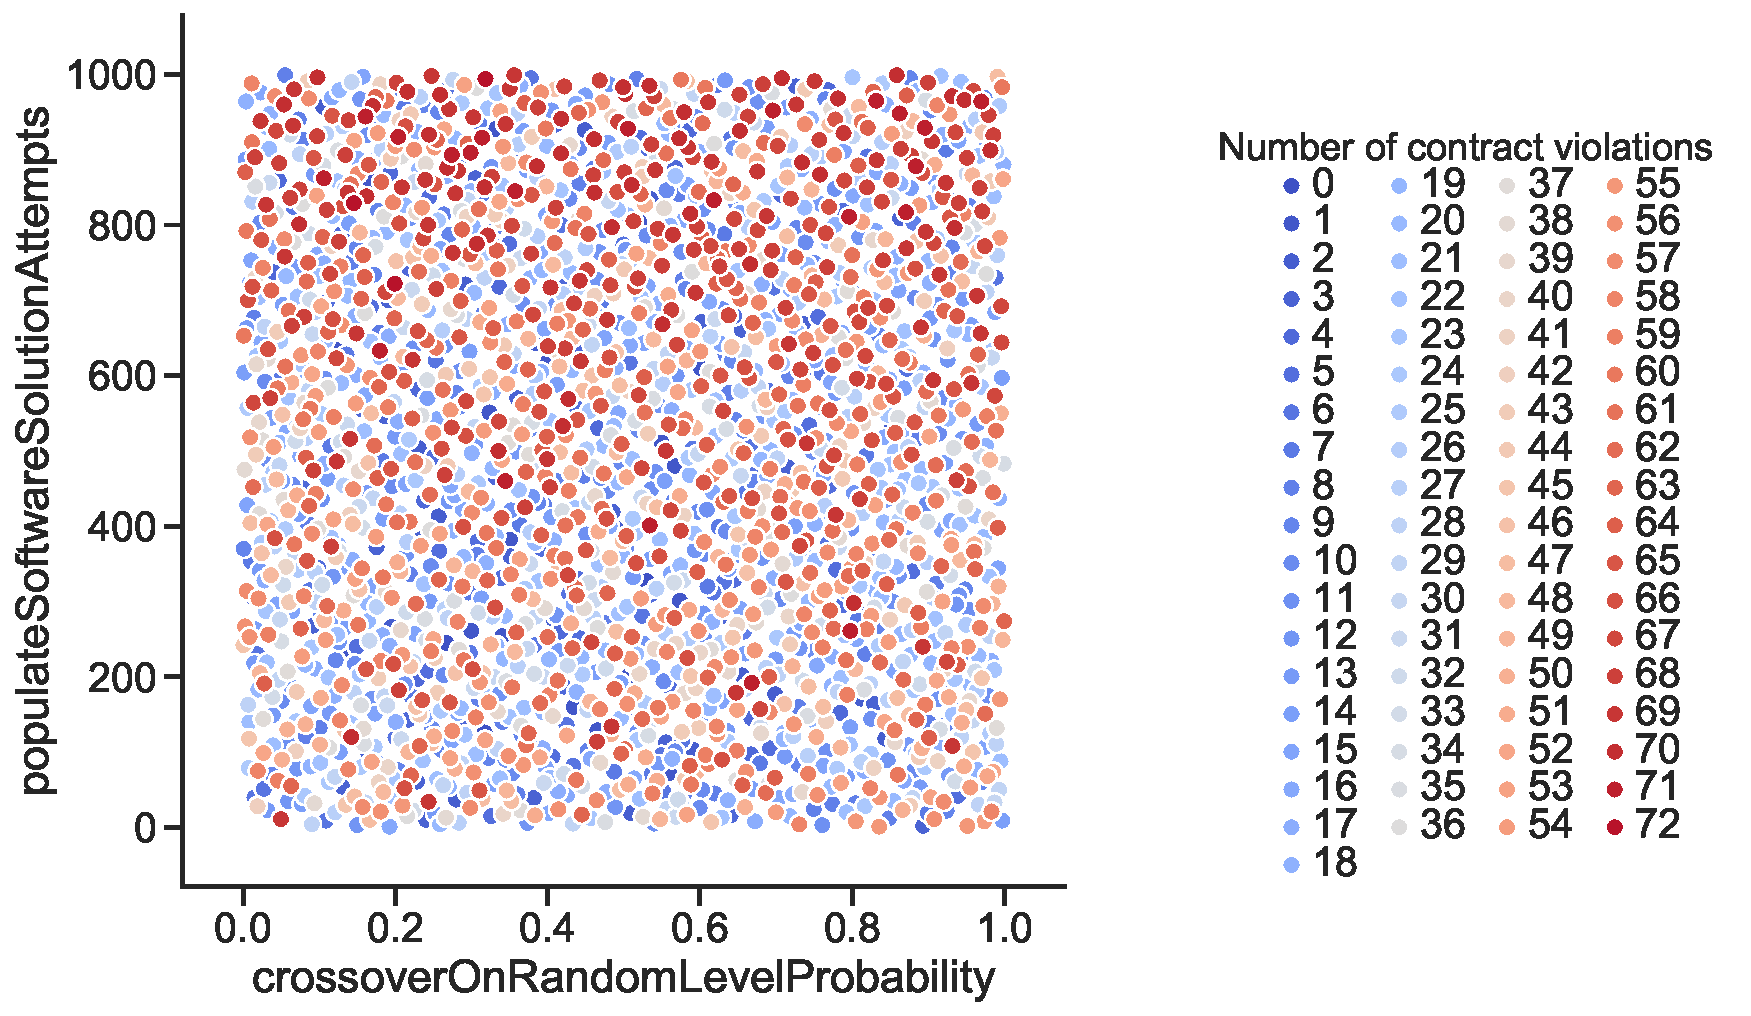
\includegraphics[width=\textwidth]{images/PairsDistr/crossoverOnRandomLevelProbability_populateSoftwareSolutionAttempts.pdf}
	\caption[]{crossoverOnRandomLevelProbability and populateSoftwareSolutionAttempts pairs distribution}
	\label{fig:crossoverOnRandomLevelProbability_populateSoftwareSolutionAttempts_pair}
\end{figure}